\documentclass{article}%
\usepackage[T1]{fontenc}%
\usepackage[utf8]{inputenc}%
\usepackage{lmodern}%
\usepackage{textcomp}%
\usepackage{lastpage}%
\usepackage[head=40pt,margin=0.5in,bottom=0.6in]{geometry}%
\usepackage{graphicx}%
%
\title{\textbf{Cañicultores piden al gobierno proteger la producción nacional}}%
\author{DICK TORRES}%
\date{23/11/2018}%
%
\begin{document}%
\normalsize%
\maketitle%
\textbf{URL: }%
http://www.eluniversal.com/economia/26484/canicultores{-}piden{-}al{-}gobierno{-}proteger{-}la{-}produccion{-}nacional\newline%
%
\textbf{Periodico: }%
EU, %
ID: %
26484, %
Seccion: %
economia\newline%
%
\textbf{Palabras Claves: }%
NO\_TIENE\newline%
%
\textbf{Derecho: }%
3.1%
, Otros Derechos: %
2.10%
, Sub Derechos: %
3.1.1, 2.10.1%
\newline%
%
\textbf{EP: }%
NO\newline%
\newline%
%
\textbf{\textit{La producción de caña molida de azúcar alcanzó este año a 3,5 millones de toneladas}}%
\newline%
\newline%
%
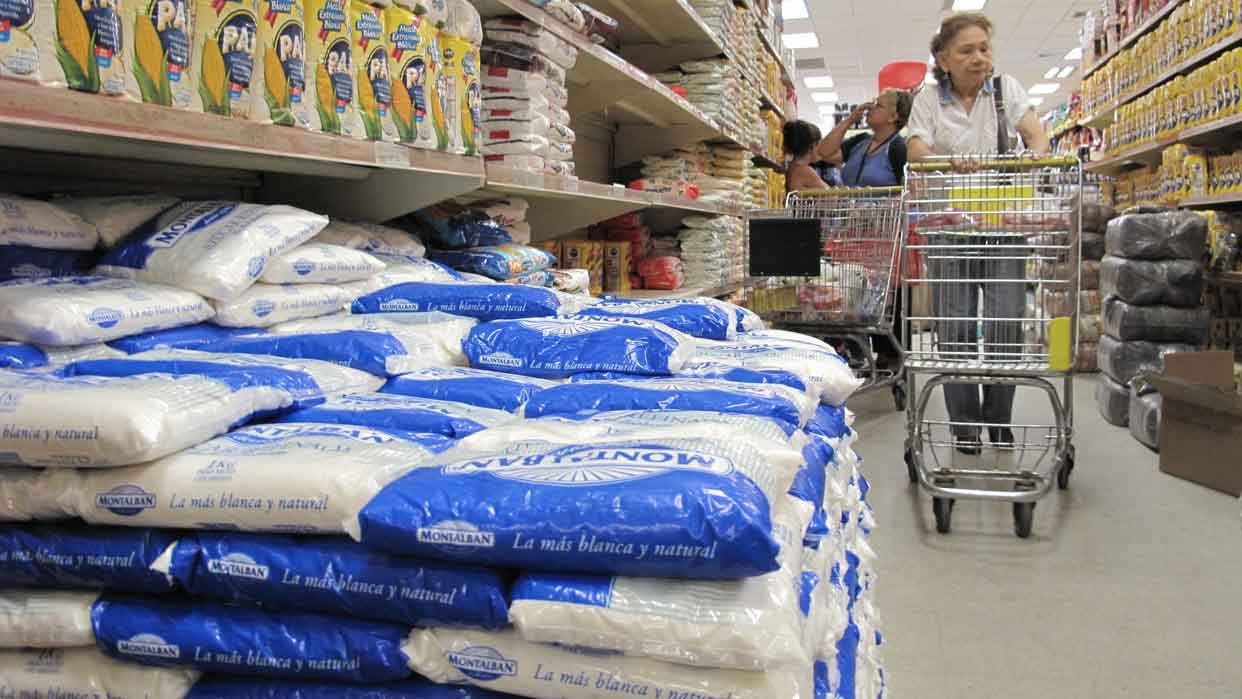
\includegraphics[width=300px]{244.jpg}%
\newline%
%
Caracas.{-} Políticas dirigidas a proteger lo hecho en Venezuela solicitaron al Gobierno Nacional los cañicultores quienes este jueves se declararon en emergencia por la caída de la producción.%
\newline%
%
En rueda de prensa, el presidente de la Federación Nacional de Asociaciones de Cañicultores (Fesoca), José Ricardo Álvarez, afirmó que la situación del sector es “difícil de mantener los cultivos con unos ingresos regulados por el problema inflacionario”.%
\newline%
%
El dirigente gremial propuso buscar correctivos en forma periódica y anclada a un precio en divisas de los países vecinos, entre ellos Colombia, para acceder a los insumos que son necesarios para las zafras.%
\newline%
%
Álvarez expresó que constantemente los directivos de la Federación que preside mantienen reuniones y conversaciones con los representantes del Gobierno de quienes afirmó “toman decisiones muy tardías en detrimento de los productores del campo venezolano”.%
\newline%
%
Sostuvo que la tardanza de las autoridades gubernamentales obedece a que “los funcionarios públicos están más pendientes de las importaciones que de lo hecho en Venezuela”.%
\newline%
%
El dirigente de los cañicultores denunció que la empresa estatal en fertilizantes Agropatria “considera que la caña de azúcar no es un producto prioritario para el país y por esa razón nos limita los insumos”.%
\newline%
%
Precisó que los cañicultores privados produjeron este año 3 millones 540 mil toneladas de caña molida que arrojaron, a su vez, 240 mil toneladas de azúcar, y estimó que el próximo  año la producción bajará a 2 millones y medio, “por falta de insumos agrícolas”.%
\newline%
%
El dirigente empresarial afirmó que el “70\% de los centrales azucareros están en manos del sector público y solo produjeron 10\%, lo equivale a unas 500 mil toneladas de caña molida de azúcar en contra de los tres millones que produjeron los cañicultores privados”.%
\newline%
%
“La caída de la producción “es una clara señal de que es el sector privado el que debe llevar a cabo las labores de producción en Venezuela”, dijo.%
\newline%
%
“Esa situación en la caída de la producción de la caña de azúcar, significa que el Gobierno Nacional seguirá importando y fortaleciendo a los productores extranjeros”, agregó.%
\newline%
%
Llamado de Fedeagro%
\newline%
%
A la rueda de prensa también asistieron dirigentes empresariales de varios estados, entre ellos Aragua, Portuguesa y Vargas. También Aquiles Hopkins, presidente de la Confederación de Asociaciones de Productores Agropecuarios (Fedeagro).%
\newline%
%
Hopkins pidió al presidente Nicolás Maduro reflexionar por considerar que el Ejecutivo Nacional no le da apoyo a “lo hecho en Venezuela”.%
\newline%
%
“Los productores de caña de azúcar y de otros rubros estamos cada día más golpeados, más mermados y cada día producen menos alimentos y las consecuencias las sufrirán los 30 millones de venezolanos”.%
\newline%
%
“Si el Gobierno no rectifica sus políticas económicas desaparecerá la producción nacional, lo cual agravará la crisis, la escasez y el desabastecimiento”, afirmó.%
\newline%
%
Hopkins responsabilizó a las políticas monetarias implementadas por la administración del presidente Maduro  por la “escalada diaria en los precios de los  alimentos”.%
\newline%
%
Observó que la producción de azúcar alcanzó un récord durante la zafra de 2006 de 9 millones 600 mil toneladas y este año  es de 3,5 millones de toneladas y vamos a dos millones y medios en 2019 “lo cual es un indicador de que las cosas se están haciendo mal”.%
\newline%
%
Aquiles Hopkins, presidente de Fedeagro, pidió al presidente Nicolás Maduro rectificar su política agrícola y pecuaria.%
\newline%
%
\end{document}